% (find-LATEX "2020-2-C3-plano-tang.tex")
% (defun c () (interactive) (find-LATEXsh "lualatex -record 2020-2-C3-plano-tang.tex" :end))
% (defun C () (interactive) (find-LATEXsh "lualatex 2020-2-C3-plano-tang.tex" "Success!!!"))
% (defun D () (interactive) (find-pdf-page      "~/LATEX/2020-2-C3-plano-tang.pdf"))
% (defun d () (interactive) (find-pdftools-page "~/LATEX/2020-2-C3-plano-tang.pdf"))
% (defun e () (interactive) (find-LATEX "2020-2-C3-plano-tang.tex"))
% (defun l () (interactive) (find-LATEX "2020-2-C3-plano-tang.lua"))
% (defun o () (interactive) (find-LATEX "2020-2-C3-plano-tang.tex"))
% (defun u () (interactive) (find-latex-upload-links "2020-2-C3-plano-tang"))
% (defun v () (interactive) (find-2a '(e) '(d)))
% (defun d0 () (interactive) (find-ebuffer "2020-2-C3-plano-tang.pdf"))
% (defun cv () (interactive) (C) (ee-kill-this-buffer) (v) (g))
%          (code-eec-LATEX "2020-2-C3-plano-tang")
% (find-pdf-page   "~/LATEX/2020-2-C3-plano-tang.pdf")
% (find-sh0 "cp -v  ~/LATEX/2020-2-C3-plano-tang.pdf /tmp/")
% (find-sh0 "cp -v  ~/LATEX/2020-2-C3-plano-tang.pdf /tmp/pen/")
%     (find-xournalpp "/tmp/2020-2-C3-plano-tang.pdf")
%   file:///home/edrx/LATEX/2020-2-C3-plano-tang.pdf
%               file:///tmp/2020-2-C3-plano-tang.pdf
%           file:///tmp/pen/2020-2-C3-plano-tang.pdf
% http://angg.twu.net/LATEX/2020-2-C3-plano-tang.pdf
% (find-LATEX "2019.mk")
% (find-CN-aula-links "2020-2-C3-plano-tang" "3" "c3m202planotang" "c3pt")

% «.video-1»			(to "video-1")
% «.video-2»			(to "video-2")
% «.video-3»			(to "video-3")
% «.video-4»			(to "video-4")
%
% «.defs»			(to "defs")
% «.title»			(to "title")
% «.exercicio-1»		(to "exercicio-1")
% «.exercicio-2»		(to "exercicio-2")
% «.geral-e-particular»		(to "geral-e-particular")
% «.material-GA»		(to "material-GA")
% «.exercicio-5»		(to "exercicio-5")
% «.bortolossi-cap-7»		(to "bortolossi-cap-7")
% «.exercicio-6»		(to "exercicio-6")
% «.exercicio-7»		(to "exercicio-7")
% «.dicas-7»			(to "dicas-7")
% «.derivs-como-triangs»	(to "derivs-como-triangs")
% «.derivs-como-triangs-2»	(to "derivs-como-triangs-2")
% «.dicas-6a-e-6d»		(to "dicas-6a-e-6d")
% «.exercicio-8»		(to "exercicio-8")
% «.exercicio-9»		(to "exercicio-9")
% «.3D-fig»			(to "3D-fig")
% «.exercicio-10»		(to "exercicio-10")
% «.2021-04-16»			(to "2021-04-16")
% «.grad-intro»			(to "grad-intro")
%
% «.djvuize»			(to "djvuize")



% «video-1»  (to ".video-1")
% (c3m202planotanga "video-1")
% (find-ssr-links "c3m202planotang" "2020-2-C3-plano-tang")
% (code-video     "c3m202planotangvideo" "$S/http/angg.twu.net/eev-videos/2020-2-C3-plano-tang.mp4")
% (find-c3m202planotangvideo "0:00")
% (find-c3m202planotangvideo "0:05" "7/abril/2021")
% (find-c3m202planotangvideo "0:11" "exercicio 2")
% (find-c3m202planotangvideo "6:33" "desses vetores todos")
% (find-c3m202planotangvideo "7:11" "dêem uma olhada nessa dica (de GA)")
% (find-c3m202planotangvideo "7:24" "no desenho geral")

% «video-2»  (to ".video-2")
% (c3m202planotanga "video-2")
% (find-ssr-links "c3m202planotang2" "2020-2-C3-plano-tang-2")
% (code-video "c3m202planotang2video" "$S/http/angg.twu.net/eev-videos/2020-2-C3-plano-tang-2.mp4")
% (find-c3m202planotang2video "0:00")
% (find-c3m202planotang2video "0:02" "14/abril/2021")
% (find-c3m202planotang2video "0:02" "vídeo bem rápido sobre o exercício 6")

% «video-3»  (to ".video-3")
% (c3m202planotanga "video-3")
% (find-ssr-links "c3m202planotang3" "2020-2-C3-plano-tang-3" "NYDkZJGZSy8")
% (code-video "c3m202planotang3video" "$S/http/angg.twu.net/eev-videos/2020-2-C3-plano-tang-3.mp4")
% (find-c3m202planotang3video "0:00" "16/abril/2021: Como visualizar derivadas")
% (find-c3m202planotang3video "0:40" "")
% (find-c3m202planotang3video "1:05" "exercicio 7")
% (find-c3m202planotang3video "1:39" "derivadas como triângulos")
% (find-c3m202planotang3video "15:35" "triângulo paralelo àquele mas deslocado")

% «video-4»  (to ".video-4")
% (c3m202planotanga "video-4")
% (find-ssr-links "c3m202planotang4" "2020-2-C3-plano-tang-4" "UVJntqN10fg")
% (code-video "c3m202planotang4video" "$S/http/angg.twu.net/eev-videos/2020-2-C3-plano-tang-4.mp4")
% (find-c3m202planotang4video "0:00" "28/abril/2021")
% (find-c3m202planotang4video "0:00" "Pra explicar os exercicios 9 e 10")
% (find-c3m202planotang4video "0:16" "diagramas pro caso geral (e pra casos particulares também)")
% (find-c3m202planotang4video "0:37" "agora passar isso pra 3D")
% (find-c3m202planotang4video "0:53" "zoom num diagrama separado")
% (find-c3m202planotang4video "1:36" "que essa base é o vetor (1,0)")
% (find-c3m202planotang4video "1:52" "exercício 9")
% (find-c3m202planotang4video "2:27" "trabalhar em cima desse diagrama daqui")
% (find-c3m202planotang4video "6:29" "vetor AI")
% (find-c3m202planotang4video "7:05" "exercício 10")
% (find-c3m202planotang4video "7:27" "ao invés de F(x,y) ele escreve F(A_0)")
% (find-c3m202planotang4video "7:49" "x em negrito")
% (find-c3m202planotang4video "8:32" "esse A_0")
% (find-c3m202planotang4video "8:43" "ou seja ele recebe uma coordenada x e uma y")
% (find-c3m202planotang4video "9:07" "já que a direção x é pra cá")
% (find-c3m202planotang4video "9:47" "a gente não sabe se é esse ou o vetor maior")
% (find-c3m202planotang4video "10:27" "como alpha é aproximadamente 4")
% (find-c3m202planotang4video "10:53" "descobrir como obter")

\documentclass[oneside,12pt]{article}
\usepackage[colorlinks,citecolor=DarkRed,urlcolor=DarkRed]{hyperref} % (find-es "tex" "hyperref")
\usepackage{amsmath}
\usepackage{amsfonts}
\usepackage{amssymb}
\usepackage{pict2e}
\usepackage[x11names,svgnames]{xcolor} % (find-es "tex" "xcolor")
\usepackage{colorweb}                  % (find-es "tex" "colorweb")
%\usepackage{tikz}
%
% (find-dn6 "preamble6.lua" "preamble0")
%\usepackage{proof}   % For derivation trees ("%:" lines)
%\input diagxy        % For 2D diagrams ("%D" lines)
%\xyoption{curve}     % For the ".curve=" feature in 2D diagrams
%
\usepackage{edrx15}               % (find-LATEX "edrx15.sty")
\input edrxaccents.tex            % (find-LATEX "edrxaccents.tex")
\input edrxchars.tex              % (find-LATEX "edrxchars.tex")
\input edrxheadfoot.tex           % (find-LATEX "edrxheadfoot.tex")
\input edrxgac2.tex               % (find-LATEX "edrxgac2.tex")
%
%\usepackage[backend=biber,
%   style=alphabetic]{biblatex}            % (find-es "tex" "biber")
%\addbibresource{catsem-slides.bib}        % (find-LATEX "catsem-slides.bib")
%
% (find-es "tex" "geometry")
\usepackage[a6paper, landscape,
            top=1.5cm, bottom=.25cm, left=1cm, right=1cm, includefoot
           ]{geometry}
%
\begin{document}

\catcode`\^^J=10
\directlua{dofile "dednat6load.lua"}  % (find-LATEX "dednat6load.lua")

%L dofile "edrxtikz.lua"             -- (find-LATEX "edrxtikz.lua")
%L dofile "edrxpict.lua"             -- (find-LATEX "edrxpict.lua")
%L dofile "2020-2-C3-plano-tang.lua" -- (find-LATEX "2020-2-C3-plano-tang.lua")
\pu

% «defs»  (to ".defs")
% (find-LATEX "edrx15.sty" "colors-2019")
\long\def\ColorRed   #1{{\color{Red1}#1}}
\long\def\ColorViolet#1{{\color{MagentaVioletLight}#1}}
\long\def\ColorViolet#1{{\color{Violet!50!black}#1}}
\long\def\ColorGreen #1{{\color{SpringDarkHard}#1}}
\long\def\ColorGreen #1{{\color{SpringGreenDark}#1}}
\long\def\ColorGreen #1{{\color{SpringGreen4}#1}}
\long\def\ColorGray  #1{{\color{GrayLight}#1}}
\long\def\ColorGray  #1{{\color{black!30!white}#1}}
\long\def\ColorBrown #1{{\color{Brown}#1}}
\long\def\ColorBrown #1{{\color{brown}#1}}
\long\def\ColorOrange#1{{\color{orange}#1}}

\long\def\ColorShort #1{{\color{SpringGreen4}#1}}
\long\def\ColorLong  #1{{\color{Red1}#1}}

\def\frown{\ensuremath{{=}{(}}}
\def\True {\mathbf{V}}
\def\False{\mathbf{F}}
\def\D    {\displaystyle}

\def\drafturl{http://angg.twu.net/LATEX/2020-2-C3.pdf}
\def\drafturl{http://angg.twu.net/2020.2-C3.html}
\def\draftfooter{\tiny \href{\drafturl}{\jobname{}} \ColorBrown{\shorttoday{} \hours}}



%  _____ _ _   _                               
% |_   _(_) |_| | ___   _ __   __ _  __ _  ___ 
%   | | | | __| |/ _ \ | '_ \ / _` |/ _` |/ _ \
%   | | | | |_| |  __/ | |_) | (_| | (_| |  __/
%   |_| |_|\__|_|\___| | .__/ \__,_|\__, |\___|
%                      |_|          |___/      
%
% «title»  (to ".title")
% (c3m202planotangp 1 "title")
% (c3m202planotanga   "title")

\thispagestyle{empty}

\begin{center}

\vspace*{1.2cm}

{\bf \Large Cálculo 3 - 2020.2}

\bsk

Aula ??: o plano tangente

\bsk

Eduardo Ochs - RCN/PURO/UFF

\url{http://angg.twu.net/2020.2-C3.html}

\end{center}

\newpage

Os exercícios de hoje são pra ajudar todo mundo a entender

e visualizar as idéias principais do capítulo 7 do

Bortolossi... antes de começar dê uma olhada nele!




\newpage

{\bf Plano tangente: definição formal}

Digamos que a superfície $S$ seja dada por:
%
% (c3m202rcadeia1p 13 "exercicio-5")
% (c3m202rcadeia1     "exercicio-5")
%
$$S = \setofxyzst{z = F(x,y)},$$

como na aula passada a partir do exercício 5:

\ssk

% http://angg.twu.net/LATEX/2020-2-C3-rcadeia1.pdf
\url{http://angg.twu.net/LATEX/2020-2-C3-rcadeia1.pdf\#page=11}

\ssk

O plano tangente à superfície $S$ no ponto $(x_0,y_0,F(x_0,y_0))$ ---

ou no ponto $(x_0,y_0)$, se a gente usar a gambiarra que nos

permite rededuzir a coordenada $z$ desse ponto a partir das

coordenadas $x$ e $y$ dele --- pode ser definido como um

plano parameterizado assim:

\newpage

{\bf Plano tangente: definição formal (2)}

\msk

$$\begin{array}{rcl}
  \vv &=& \VEC{1,0,\frac{∂z}{∂x}} \\
    % &=& \VEC{1,0,\frac{∂z}{∂x}(x_0,y_0)} \\
      &=& \VEC{1,0,F_x} \\
      &=& \VEC{1,0,F_x(x_0,y_0)} \\
  \ww &=& \VEC{0,1,\frac{∂z}{∂y}} \\
    % &=& \VEC{0,1,\frac{∂z}{∂y}(x_0,y_0)} \\
      &=& \VEC{0,1,F_y} \\
      &=& \VEC{0,1,F_y(x_0,y_0)} \\
  P(t,u) &=& (x_0,y_0,z_0) + t\vv + u\ww \\
  π &=& \setofst{P(t,u)}{t,u∈\R} \\
    &=& \setofst{(x_0,y_0,z_0) + t\VEC{1,0,\frac{∂z}{∂x}} + u\VEC{0,1,\frac{∂z}{∂y}}}{t,u∈\R} \\
  \end{array}
$$

\newpage

Nós vamos começar entendendo isto em casos nos quais a

superfície $S$ é um plano... mas primeiro vamos fazer alguns

exercícios de desenhar os diagramas de numerozinhos e

algumas curvas de nível de planos.


\msk

% «exercicio-1»  (to ".exercicio-1")
% (c3m202planotangp 5 "exercicio-1")
% (c3m202planotanga   "exercicio-1")

{\bf Exercício 1.}

Em cada um dos casos abaixo a função $F$ vai ser definida por
%
$$F(x,y) = a + b·(x-x_0) + c·(y-y_0).$$

Represente graficamente em 3D os pontos da superfície $S$

associados aos pontos

$(x_0,y_0), (x_0+1,y_0), (x_0,y_0+1), (x_0+1,y_0+1)$.

Além disso faça o diagrama de numerozinhos da $F$ e

desenhe no plano $(x,y)$ pelo menos duas curvas de

nível da função $F$.


\newpage

{\bf Exercício 1 (cont.)}

a) $(x_0,y_0) = (4,2)$, $a=2$, $b=1$, $c=0$.

b) $(x_0,y_0) = (4,2)$, $a=2$, $b=0$, $c=1$.

c) $(x_0,y_0) = (4,2)$, $a=2$, $b=1$, $c=1$.

d) $(x_0,y_0) = (4,2)$, $a=2$, $b=2$, $c=-1$.

e) $(x_0,y_0) = (3,3)$, $a=2$, $b=2$, $c=-1$.


\newpage

Agora vamos recuar um pouco e fazer uns exercícios

sobre planos, sem considerá-los como planos tangentes

a alguma superfície não-plana...

\bsk

% «exercicio-2»  (to ".exercicio-2")
% (c3m202planotangp 7 "exercicio-2")
% (c3m202planotanga   "exercicio-2")

{\bf Exercício 2.}

Sejam $π_1, π_2, π_3$ estes planos aqui:
%
$$\begin{array}{rcl}
  π_1 &=& \setofxyzst{x + y + z = 2} \\
  π_2 &=& \setofxyzst{\frac{x}{2} + \frac{y}{3} + \frac{z}{6} = 1} \\
  π_3 &=& \setofxyzst{\frac{x}{2} - \frac{y}{3} + \frac{z}{6} = 1} \\
  \end{array}
$$

Para cada um destes planos encontre:

a) um ponto da forma $(x,0,0)$ pertencente a ele,

b) um ponto da forma $(0,y,0)$ pertencente a ele,

c) um ponto da forma $(0,0,z)$ pertencente a ele,

E use isto para desenhar estes planos em 3D, em

perspectiva (improvisada, à mão, sem régua).

\newpage

{\bf Exercício 2 (cont.)}

Para cada um dos planos $π_1, π_2, π_3$, do slide anterior, diga:

d) um vetor não-nulo da forma $\VEC{x,y,0}$ paralelo a ele,

e) um vetor não-nulo da forma $\VEC{x,0,z}$ paralelo a ele,

f) um vetor não-nulo da forma $\VEC{0,y,z}$ paralelo a ele,

g) um vetor da forma $\VEC{1,0,z}$ paralelo a ele,

h) um vetor da forma $\VEC{0,1,z}$ paralelo a ele,

i) um vetor da forma $\VEC{1,y,0}$ paralelo a ele.

\msk

As dicas pra fazer tudo isso visualmente estão no próximo slide.

\msk

{\bf Importante:} tente representar os itens (a) até (i) do plano
$π_1$

num desenho só em perspectiva improvisada, os itens (a) até (i)

do $π_2$ num segundo desenho, e os itens (a) até (i) do $π_3$ num

terceiro desenho.


\newpage

{\bf Exercício 2: dica 1}

Nós estamos fazendo nossos desenhos 3D usando eixos em

duas posições diferentes, como abaixo. Alguns itens vão ser

mais fáceis de desenhar numa posição, outros noutra.

% (find-latexscan-links "C3" "20210407_eixos")
% (find-xpdf-page "~/LATEX/2020-2-C3/20210407_eixos.pdf")
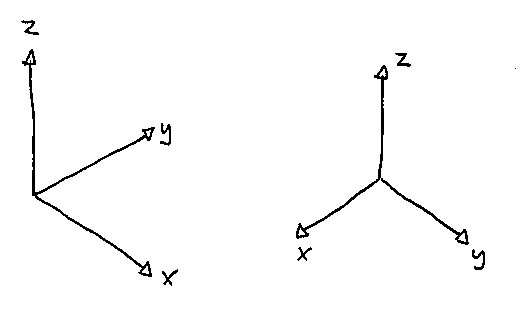
\includegraphics[height=5cm]{2020-2-C3/20210407_eixos.pdf}


\newpage

% «geral-e-particular»  (to ".geral-e-particular")
% (c3m202planotangp 10 "geral-e-particular")
% (c3m202planotanga    "geral-e-particular")

{\bf Exercício 2: dica 2}

Quando os livros de GA fazem um desenho que parece ser um

caso geral na verdade eles usam um caso particular disfarçado...

Por exemplo:

\bsk

$
% (find-latexscan-links "C3" "20210407_vetores_caso_geral")
% (find-xpdf-page "~/LATEX/2020-2-C3/20210407_vetores_caso_geral.pdf")
\myvcenter{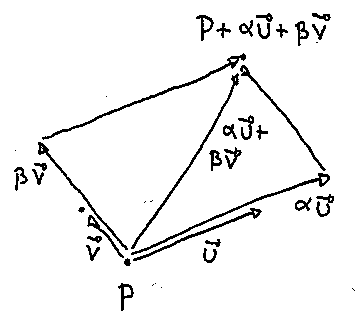
\includegraphics[height=4.5cm]{2020-2-C3/20210407_vetores_caso_geral.pdf}}
\quad
$⇒$
\quad
% (find-latexscan-links "C3" "20210407_vetores_caso_particular")
% (find-xpdf-page "~/LATEX/2020-2-C3/20210407_vetores_caso_particular.pdf")
\myvcenter{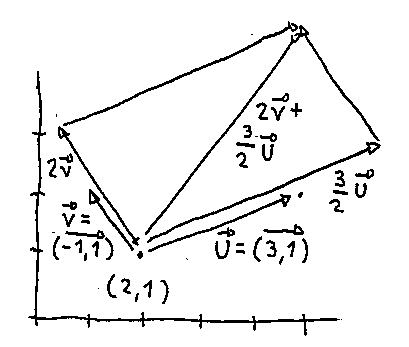
\includegraphics[height=4.5cm]{2020-2-C3/20210407_vetores_caso_particular.pdf}}
$

\newpage

{\bf Exercício 3.}

Assista este vídeo aqui:

\ssk

{\footnotesize

\url{http://angg.twu.net/eev-videos/2020-2-C3-plano-tang.mp4}

}

\ssk

E faça o ``caso geral'' ao qual ele se refere.

Mais precisamente: seja $π_4$ um plano que contém os pontos

$(a,0,0)$, $(0,b,0)$, $(0,0,c)$, e faça os itens (a) até (i)

do exercício 2 para este plano $π_4$.


\newpage

{\bf Exercício 4.}

Sejam $P=(0,0,a)$, $\vv = \VEC{1,0,b}$, $\ww = \VEC{0,1,c}$, e:
%
$$\begin{array}{rcl}
  π_5 &=& \setofst{P+\aa\vv+\bb\ww}{α,β∈\R} \\
      &=& \setofst{(0,0,a)+\aa\VEC{1,0,b}+\bb\VEC{0,1,c}}{α,β∈\R} \\
  \end{array}
$$

a) Encontre um ponto de $π_6$ da forma $(x,0,0)$.

b) Encontre um ponto de $π_6$ da forma $(0,y,0)$.

c) Encontre um ponto de $π_6$ da forma $(0,0,z)$.

\msk

d) Represente graficamente, num gráfico só com

perspectiva improvisada: $P$, $P+\vv$, $P+\ww$,

e os pontos dos seus itens (a), (b) e (c).

\msk

e) Complete as lacunas com as fórmulas certas:
%
$$\begin{array}{rcl}
  π_5 % &=& \setofst{P+\aa\vv+\bb\ww}{α,β∈\R} \\
      &=& \setofst{(0,0,a)+\aa\VEC{1,0,b}+\bb\VEC{0,1,c}}{α,β∈\R} \\
      &=& \setofxyzst{z = ▁ + ▁x + ▁y} \\
  \end{array}
$$




\newpage

% «material-GA»  (to ".material-GA")
% (c3m202planotangp 13 "material-GA")
% (c3m202planotanga    "material-GA")

{\bf Material de Geometria Analítica}

No tempo em que dei Geometria Analítica eu preparei um monte

de material com exercícios parecidos com os que vocês acabaram

de fazer, em que a gente começava por casos particulares com

contas fáceis e que eram fáceis de desenhar e aí a gente

generalizava eles... o link pra esse material está aqui:

\ssk

\url{http://angg.twu.net/LATEX/material-para-GA.pdf}

\ssk

Talvez eu peça pra vocês fazerem alguns exercícios dele depois...



\newpage

% «exercicio-5»  (to ".exercicio-5")
% (c3m202planotangp 14 "exercicio-5")
% (c3m202planotanga    "exercicio-5")

O melhor modo de desenhar planos em $\R^3$ é desenhando as interseções
desse plano com os planos $π_{xy}$, $π_{xz}$, e $π_{yz}$, ou pedaços
dessas interseções. Nos exercícios anteriores nós fizemos isto pra
planos da forma
%
$$\setofxyzst{\textstyle \frac xa + \frac yb + \frac zc = 0},$$
%
em que desenhamos a interseção deles com um octante do $\R^3$, que era
um triângulo. Agora vamos ver planos que contêm retas parelelas aos
eixos.

Lembre que você pode desenhar as suas perspectivas de
jeitos bem improvisados, desde que as coordenadas dos pontos estejam
claras... e lembre que o Danilo Pereira, que fez o vídeo que eu
recomendei no mini-teste 2, usa uma perspectiva bem tosca, que não é
isométrica! Links:

\ssk

{\footnotesize

% https://pt.wikipedia.org/wiki/Perspectiva_isom%C3%A9trica
\url{https://pt.wikipedia.org/wiki/Perspectiva_isom\%C3\%A9trica}

\url{https://pt.wikipedia.org/wiki/Octante_(geometria_espacial)}

}

\bsk

{\bf Exercício 5.}

Represente graficamente os planos abaixo (em $\R^3$).

Considere que $a,b,c>0$. 

a) $π_7 = \setofxyzst{\frac ax + \frac by = 1}$

b) $π_8 = \setofxyzst{\frac ax + \frac cz = 1}$

c) $π_9 = \setofxyzst{\frac by + \frac cz = 1}$




\newpage

% «bortolossi-cap-7»  (to ".bortolossi-cap-7")
% (c3m202planotangp 16 "bortolossi-cap-7")
% (c3m202planotanga    "bortolossi-cap-7")

No mini-teste 2 você deve ter aprendido a representar graficamente
vários tipos de objetos em $\R^3$, tanto em casos particulares quanto
em casos gerais... agora vamos usar isto pra entender como o
Bortolossi define a derivada de uma função de $\R^m$ em $\R^n$ usando
a matriz Jacobiana, no capítulo 7, na página 256.

Vamos começar entendendo o que ele faz no início do capítulo 7, em que
ele considera uma função de $\R^1$ em $\R^1$.

% (find-bortolossi7page (+ -238 256) "matriz jacobiana")


\newpage

% «exercicio-6»  (to ".exercicio-6")
% (c3m202planotangp 17 "exercicio-6")
% (c3m202planotanga    "exercicio-6")

{\bf Exercício 6.}

$
% (find-latexscan-links "C3" "20210414_bortolossi_p240_a_b")
% (find-xpdf-page "~/LATEX/2020-2-C3/20210414_bortolossi_p240_a_b.pdf")
\myvcenter{
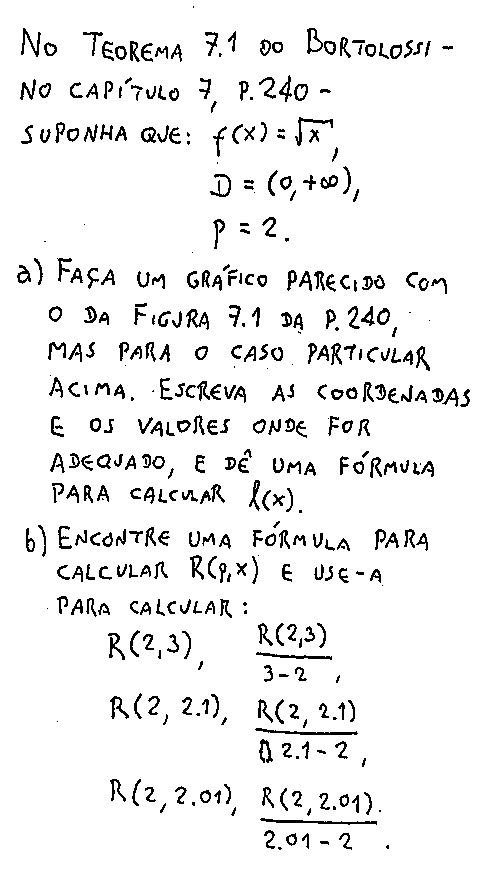
\includegraphics[height=7.2cm]{2020-2-C3/20210414_bortolossi_p240_a_b.pdf}
}
\qquad
%
% (find-latexscan-links "C3" "20210414_bortolossi_p240_c")
% (find-xpdf-page "~/LATEX/2020-2-C3/20210414_bortolossi_p240_c.pdf")
\myvcenter{
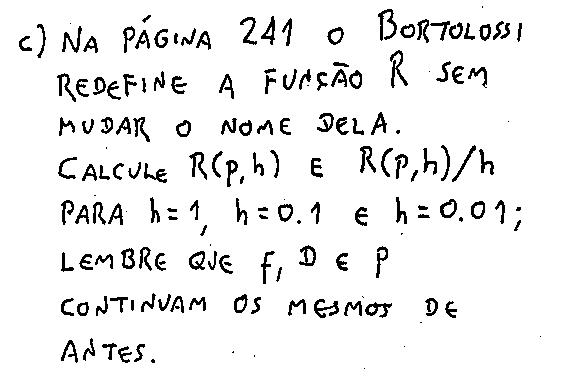
\includegraphics[height=3cm]{2020-2-C3/20210414_bortolossi_p240_c.pdf}
}
$

\newpage

{\bf Exercício 6 (cont.)}

% (find-latexscan-links "C3" "20210414_bortolossi_p240_d_e")
% (find-xpdf-page "~/LATEX/2020-2-C3/20210414_bortolossi_p240_d_e.pdf")
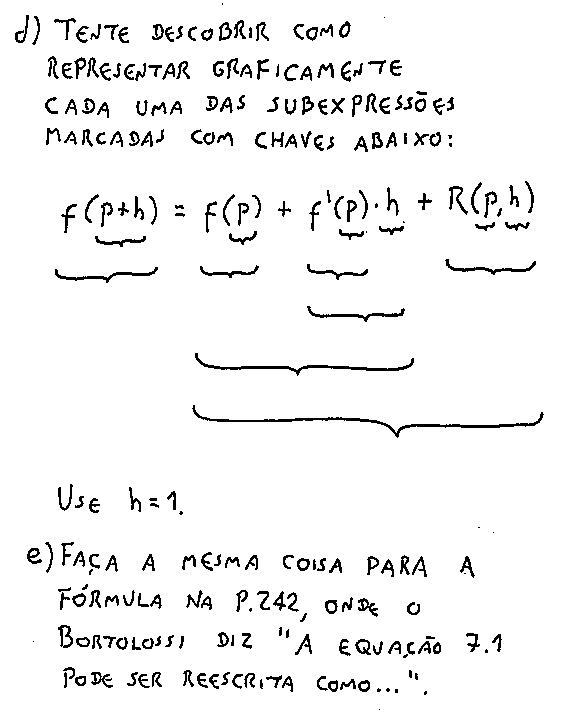
\includegraphics[height=7cm]{2020-2-C3/20210414_bortolossi_p240_d_e.pdf}

\newpage

Agora vamos tentar entender a seção ``Funções vetoriais:

o caso geral'' do Bortolossi, que começa na p.253.

\bsk

% «exercicio-7»  (to ".exercicio-7")
% (c3m202planotangp 19 "exercicio-7")
% (c3m202planotanga    "exercicio-7")

{\bf Exercício 7.}

Leia ela até a página 255. Suponha que $n=2$, $m=1$,

$D=\R^2$, $𝐛p=(2,3)$, $𝐛x=(42,99)$.

a) Simplifique o máximo possível a definição do $D𝐛f(𝐛p)$

neste caso. O resultado vai dar ou uma matriz $2×1$ ou

uma matriz $1×2$.

b) Simplifique o máximo possível a fórmula (7.6) da

página 255, que é:
%
$$𝐛f(𝐛x) = 𝐛f(𝐛p) + D𝐛f(𝐛p)·(𝐛x-𝐛p) + 𝐛R(𝐛p,𝐛x)$$

Esse `$·$' é uma multiplicação de matrizes.

c) Faça o mesmo para a fórmula no início da página 256.

\newpage

% «dicas-7»  (to ".dicas-7")
% (c3m202planotangp 20 "dicas-7")
% (c3m202planotanga    "dicas-7")
% (find-fline "~/2020.2-C2/tmp/")
% (find-fline "~/2020.2-C2/tmp/20210416_C3_dica_bortolossi.jpg")
% (find-bortolossi7page (+ -238 256)    "matriz jacobiana")

{\bf Dicas pro exercício 7}

Se $m=3$ e $n=4$ então a matriz jacobiana da p.256

do Bortolossi vira isso aqui:

\def\fxp#1#2{\frac{∂f_#1}{∂x_#2}(𝐛p)}

$$D𝐛f(𝐛p) =
  \bmat{
  \fxp11 & \fxp12 & \fxp13 & \fxp14 \\[5pt]
  \fxp21 & \fxp22 & \fxp23 & \fxp24 \\[5pt]
  \fxp31 & \fxp32 & \fxp33 & \fxp34 \\
  }_{3×4} \;,
$$

e: \;\;
   $𝐛x-𝐛p = \bmat{x_1 \\ x_2 \\ x_3 \\ x_4} -  
             \bmat{p_1 \\ p_2 \\ p_3 \\ p_4}
           = \bmat{x_1-p_1 \\ x_2-p_2 \\ x_3-p_3 \\ x_4-p_4}
$

\msk
\msk

compare com o que aparece no início da p.255, e veja que

sabendo $m$ e $n$ a gente consegue se livrar das reticências...




\newpage

% «exercicio-8»  (to ".exercicio-8")
% (c3m202planotangp 20 "exercicio-8")
% (c3m202planotanga    "exercicio-8")
% (find-bortolossi7page (+ -238 242) "7.2. Aproximação linear em Cálculo 2")

{\bf Exercício 8.}

Digamos que $π$ seja o plano que passa pelos pontos

$(a,0,0)$, $(0,b,0)$, $(0,0,c)$ --- o do mini-teste.

\msk

Na seção 7.2 do Bortolossi ele diz que um certo plano

tangente a uma superfície é:
%
$$z = l(x,y) = α + β·x + γ·y$$

Digamos que esse plano $z = l(x,y)$ seja o nosso plano

$π$, que passa por $(a,0,0)$, $(0,b,0)$, $(0,0,c)$.

\msk

a) Quem são $α$, $β$, e $γ$?

b) Quem são as derivadas parciais da função $l$?


\newpage

% «derivs-como-triangs»  (to ".derivs-como-triangs")
% (c3m202planotangp 22 "derivs-como-triangs")
% (c3m202planotanga    "derivs-como-triangs")

{\bf Derivadas como triângulos}

Vamos voltar ao início do capítulo 7 do Bortolossi um pouco.

Nós podemos interpretar a derivada de uma função $f:\R→\R$

num ponto $p∈\R$, $f'(p)$, como uma razão entre distâncias

hortizontais e distncias verticais. Por exemplo, nós já vimos

esta fórmula várias vezes,
%
$$Δy = f'(p)Δx$$

às vezes com `$≈$', às vezes com `$=$'... e já vimos o que

quer dizer geometricamente nós termos $f'(p)=\frac12$, $f'(p)=2$,

$f'(p)=-1$...

\newpage

% «derivs-como-triangs-2»  (to ".derivs-como-triangs-2")
% (c3m202planotangp 23 "derivs-como-triangs-2")
% (c3m202planotanga    "derivs-como-triangs-2")

{\bf Derivadas como triângulos (2)}

Existem muitos jeitos de representar graficamente algo

como ``$f'(p) = \frac12$''. Um deles é representar cada $f'(p)$

como um triângulo retângulo como o abaixo,

% (find-latexscan-links "C3" "20210416_fp")
% (find-xpdf-page "~/LATEX/2020-2-C3/20210416_fp.pdf")
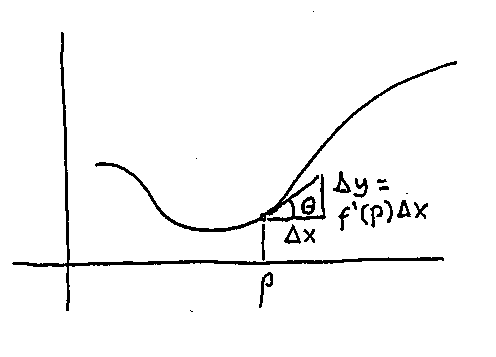
\includegraphics[height=4cm]{2020-2-C3/20210416_fp.pdf}

com  o vértice esquerdo no ponto $(p,f(p))$, e com o cateto

de baixo medindo $Δx$ e o cateto da direita medindo $Δy$...

\ssk

Às vezes isto é bem melhor que visualizar $f'(p)$ como $\tanθ$.


\newpage

% «dicas-6a-e-6d»  (to ".dicas-6a-e-6d")
% (c3m202planotangp 24 "dicas-6a-e-6d")
% (c3m202planotanga    "dicas-6a-e-6d")

{\bf Dicas sobre os exercícios 6a e o 6d}

Na aula de 18/abril quando nós estávamos discutindo o exercício 6a no
Telegram algumas pessoas viram que era muito difícil fazer o diagrama
direito, porque elas teriam que desenhar muitos objetos juntos numa
área pequena do diagrama... aí eu mandei a sugestão do próximo slide,
em que uma parte do diagrama é representada várias vezes em lugares
diferentes do papel, cada vez com detalhes diferentes sendo
indicados...

Lembre da dica 7 daqui:

% \ssk

{\footnotesize

% http://angg.twu.net/LATEX/material-para-GA.pdf#page=5
\url{http://angg.twu.net/LATEX/material-para-GA.pdf\#page=5}

}

\ssk

Quando não funciona bem fazer um diagrama do jeito mais óbvio a gente
pode improvisar um pouco, desde que os leitores consigam entender o
que a gente fez.



\newpage

% (find-latexscan-links "C3" "20210428_C3_6a")
% (find-xpdf-page "~/LATEX/2020-2-C3/20210428_C3_6a.pdf")
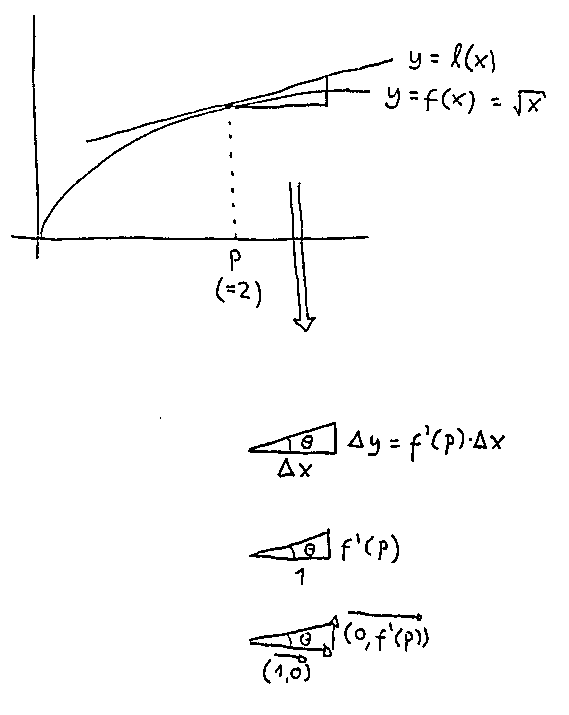
\includegraphics[height=8cm]{2020-2-C3/20210428_C3_6a.pdf}


\newpage

% «exercicio-9»  (to ".exercicio-9")
% (c3m202planotangp 26 "exercicio-9")
% (c3m202planotanga    "exercicio-9")

{\bf Dicas sobre os exercícios 6a e o 6d (cont.)}

Quando o curso de Cálculo 3 era presencial era fácil pôr as pessoas
pra discutirem em grupo pra entenderem as convenções dos diagramas dos
livros e pra encontrarem jeitos de desenhar novos diagramas que os
colegas achassem bons...

\msk

Eu ainda não sei fazer algo assim acontecer por Telegram ${=}($

\msk

{\bf Exercício 9}

O diagrama do próximo slide é uma tentativa de adaptar o diagram do
slide anterior --- da dica do exercício 6a --- para algo 3d. Eu ainda
não sei fazer esses diagramas direito no computador, então à direita
do diagrama feito por computador eu pus uma versão dele feita à mão
com os nomes dos pontos. Digamos que $A=(x_0,y_0,z_0)$, e que
$\Vec{AE} = \VEC{1,0,F_x(x_0,y_0)}$ e $\Vec{AG} =
\VEC{0,1,F_y(x_0,y_0)}$. Descubra as coordenadas dos pontos
$B,C,D,E,F,G,H,I$.



\newpage

% «3D-fig»  (to ".3D-fig")
% (c3m202planotangp 27 "3D-fig")
% (c3m202planotanga    "3D-fig")
% (find-es "ipython" "perspective")

% (find-LATEX "edrxgac2.tex" "beginpicture")
\def\pictgray#1{{\color{GrayPale}\linethickness{0.3pt}#1}}

%L rv = savevars(function (...)
%L      ex,ey,vx,vy, A0, A,B,C,D,E,F,E,G = ... end,
%L      ex,ey,vx,vy, A0, A,B,C,D,E,F,E,G)
%L
%L ex = v3(1,0,0)
%L ey = v3(0,1,0)
%L vx = v3(0,0,0.5)
%L vy = v3(0,0,1.5)
%L vz = v3(0,0,0.5)
%L A0 = v3(2,1,0); B0 = A0 + ex; C0 = A0 + ey; D0 = B0 + ey
%L A  = A0 + vz
%L B  = A + ex
%L C  = A + ey
%L D  = A + ex + ey
%L E  = B + vx
%L F  = E + ey
%L G  = C + vy
%L H  = G + ex
%L I  = H + vx
%L
%L V3.__index.p1 = V{2,-0.5}
%L V3.__index.p2 = V{1,1.25}
%L
\pu

$%\bhbox{$
 \vcenter{\hbox{%
 \unitlength=20pt
 \beginpicture(0,-4)(8,8)
%P \pictgray{<v3():xygrid(3,3)>}
%P <v3():axeswithticks(3,3,3)>
%P \pictgray{\Line<A0><A> \Line<B0><B> \Line<C0><C> \Line<D0><D>}
%P \Line<A><B><D><C><A>
%P \Line<A><E><B> \Line<E><F><I><E>
%P \Line<A><G><C> \Line<G><H><I><G>
%P \Line<D><F>
 \pu
 \end{picture}%
 }}
 %$}
 %
 \qquad
 % (find-latexscan-links "C3" "20210428_C3_exercicio_9")
 % (find-xpdf-page "~/LATEX/2020-2-C3/20210428_C3_exercicio_9.pdf")
 \myvcenter{
 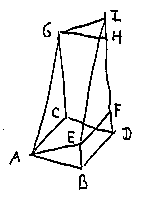
\includegraphics[height=5cm]{2020-2-C3/20210428_C3_exercicio_9.pdf}
 }
$
%

%L rv()
\pu

% Falta:
%\put(3,6.25){\cell{(3,6)}}%
%\put(8,0.75){\cell{(8,1)}}%





\newpage

% «exercicio-10»  (to ".exercicio-10")
% (c3m202planotangp 28 "exercicio-10")
% (c3m202planotanga    "exercicio-10")

{\bf Exercício 10.}

(Este exercício generaliza as idéias do 9).

\ssk

Sejam:
%
$$\begin{array}{rcl}
  F &:& \R^2 → \R, \\
  S &=& \setofxyzst{z=F(x,y)}, \\
  A_0 &=& (x_0,y_0), \\
  A &=& (x_0,y_0,F(x_0,y_0)), \\
  \vv &=& \VEC{1,0,F_x(A_0)}, \\
  \ww &=& \VEC{0,1,F_y(A_0)}, \\
  α,β &∈& \R. \\
  \end{array}
$$

a) Identifique no diagrama do próximo slide os pontos:

$A+\vv$, $A+\aa\vv$, $A+\ww$, $A+\bb\ww$, $A+\aa\vv+\bb\ww$, 

Dica: $α$ é aproximadamente 4, e $β$ aproximadamente 2.5.

\newpage

% (find-latexscan-links "C3" "20210428_C3_exercicio_10")
% (find-xpdf-page "~/LATEX/2020-2-C3/20210428_C3_exercicio_10.pdf")
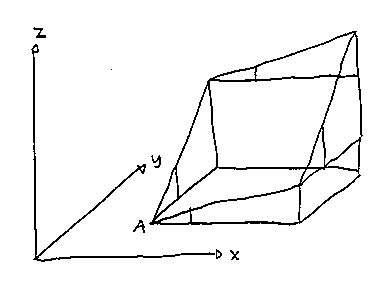
\includegraphics[height=8cm]{2020-2-C3/20210428_C3_exercicio_10.pdf}


\newpage

{\bf Exercício 10 (cont.)}

\msk

b) Verifique -- visualmente -- que os pontos

$A+\vv$, $A+\aa\vv$, $A+\ww$, $A+\bb\ww$, $A+\aa\vv+\bb\ww$, 

do item (a) estão todos no mesmo plano.

\msk

c) Verifique que esse plano é o plano tangente

à superfície $S$ no ponto $A$.


\newpage

% «2021-04-16»  (to ".2021-04-16")
% (find-fline "~/2020.2-C2/tmp/" "20210416_C3_derivada_triangulo.jpg")
% (find-fline "~/2020.2-C2/tmp/" "20210416_C3_derivada_triangulos.jpg")
% (find-fline "~/2020.2-C3/C3-M1-RCN-PURO-2020.2/" "messages3.html")
% (kill-new "14 April 2021")
% (kill-new "16 April 2021")

\newpage

% «grad-intro»  (to ".grad-intro")
% (c3m202planotangp 31 "grad-intro")
% (c3m202planotanga    "grad-intro")

{\bf Introdução ao vetor gradiente}

...então, primeiro eu preciso que voces relembrem dessa figura e
encontrem uma fórmula pra função $F(x,y)$, e depois calculem as
derivadas parciais $F_x(x_0,y_0)$ e $F_y(x_0,y_0)$ - elas devem dar
expressões que não dependem dos valores de $x_0$ e $y_0$.

% (find-latexscan-links "C3" "20210430_grad_superficie_orig")
% (find-xpdf-page "~/LATEX/2020-2-C3/20210430_grad_superficie_orig.pdf")
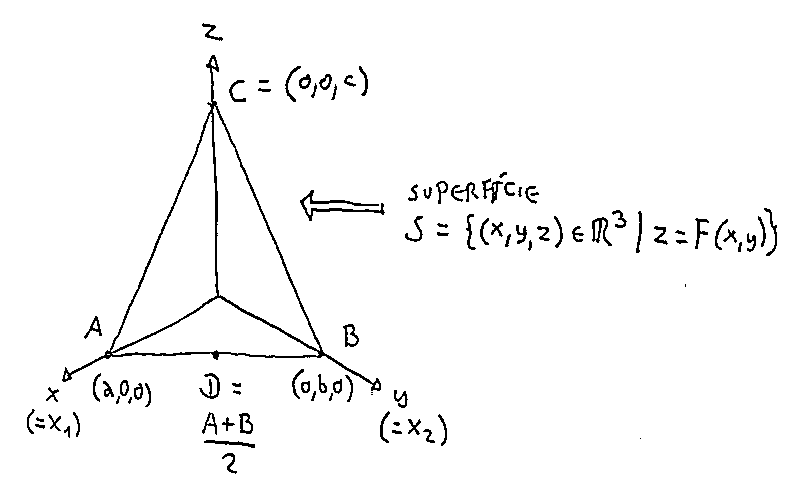
\includegraphics[height=5cm]{2020-2-C3/20210430_grad_superficie_orig.pdf}

\newpage

\begin{tabular}[c]{c}
%
% (find-latexscan-links "C3" "20210430_grad_notacao_bort")
% (find-xpdf-page "~/LATEX/2020-2-C3/20210430_grad_notacao_bort.pdf")
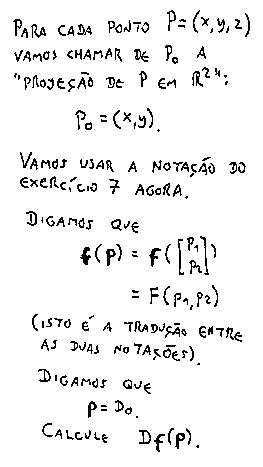
\includegraphics[height=6.5cm]{2020-2-C3/20210430_grad_notacao_bort.pdf}
\\
O resultado disso deve \\
dar uma matrix $2×1$.
\end{tabular}
%
\qquad
%
\begin{tabular}[c]{c}
% (find-latexscan-links "C3" "20210430_grad_leia_a_definicao")
% (find-xpdf-page "~/LATEX/2020-2-C3/20210430_grad_leia_a_definicao.pdf")
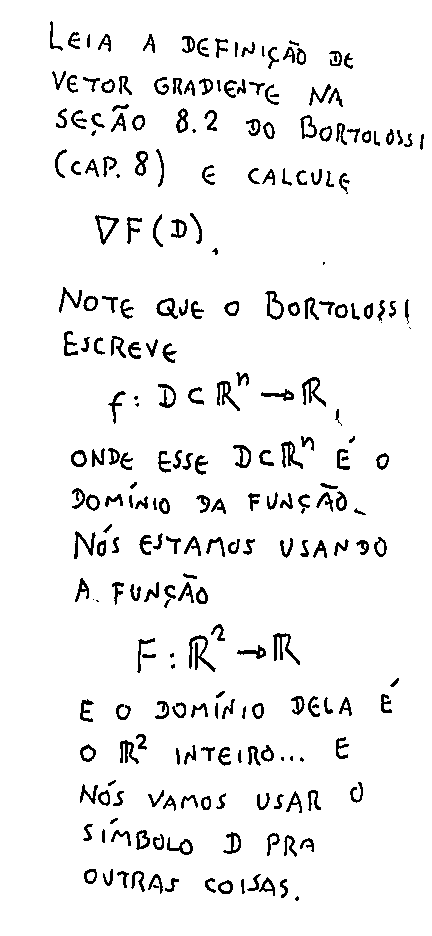
\includegraphics[height=8cm]{2020-2-C3/20210430_grad_leia_a_definicao.pdf}
\end{tabular}

\newpage

\vspace*{-1cm}

\begin{tabular}[c]{c}
% (find-latexscan-links "C3" "20210430_grad_444_intro")
% (find-xpdf-page "~/LATEX/2020-2-C3/20210430_grad_444_intro.pdf")
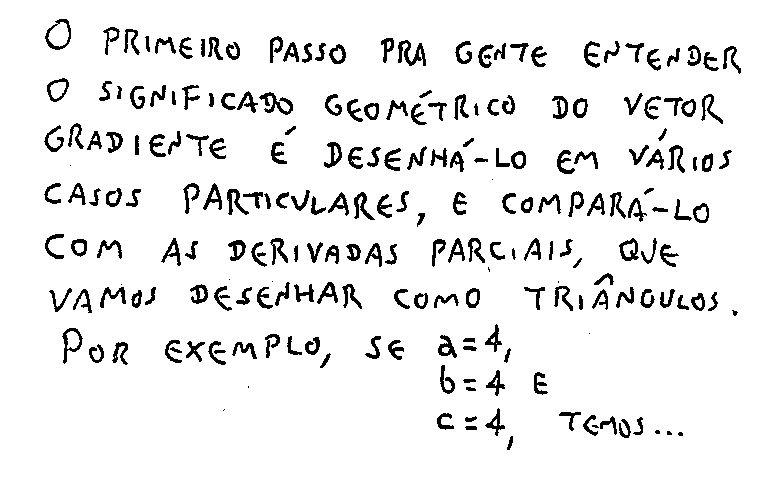
\includegraphics[height=3cm]{2020-2-C3/20210430_grad_444_intro.pdf}
\\[-10pt]
% (find-latexscan-links "C3" "20210430_grad_444")
% (find-xpdf-page "~/LATEX/2020-2-C3/20210430_grad_444.pdf")
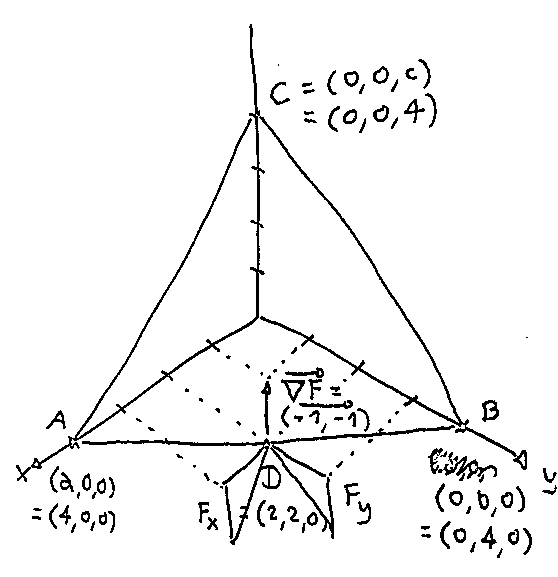
\includegraphics[height=6.0cm]{2020-2-C3/20210430_grad_444.pdf}
\end{tabular}
%
\quad
%
\begin{tabular}[c]{c}
% (find-latexscan-links "C3" "20210430_grad_422")
% (find-xpdf-page "~/LATEX/2020-2-C3/20210430_grad_422.pdf")
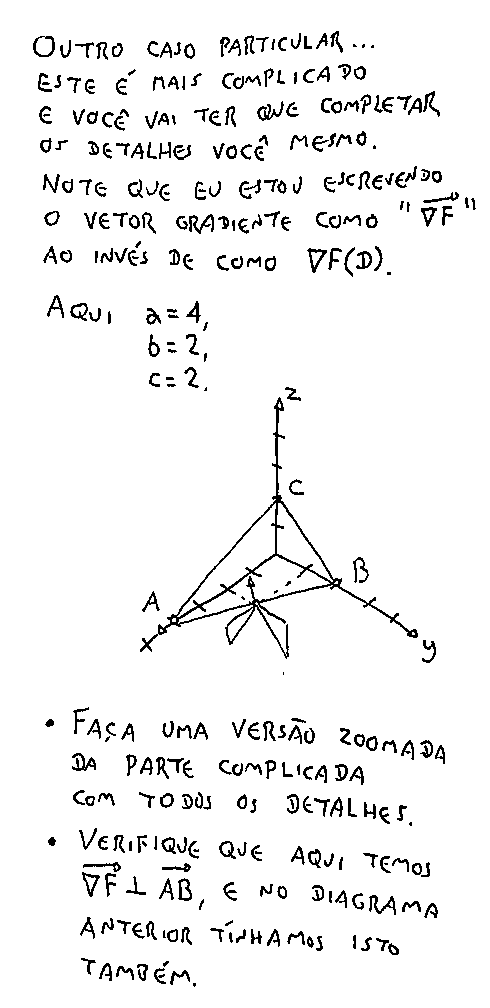
\includegraphics[height=9cm]{2020-2-C3/20210430_grad_422.pdf}
\end{tabular}

\newpage

%
\qquad
%
% (find-latexscan-links "C3" "20210430_grad_423")
% (find-xpdf-page "~/LATEX/2020-2-C3/20210430_grad_423.pdf")
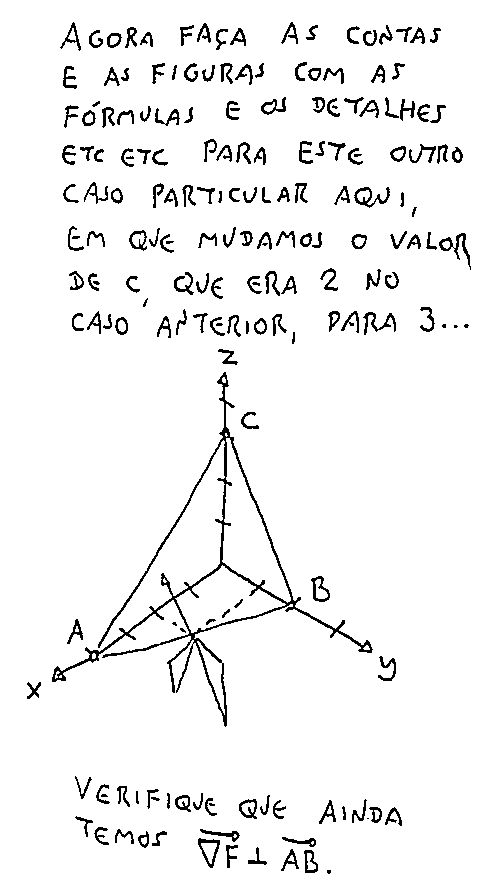
\includegraphics[height=8cm]{2020-2-C3/20210430_grad_423.pdf}




% (find-bortolossi7page (+ -238 239) "7. Aproximação linear e a regra da cadeia")





%\printbibliography

\GenericWarning{Success:}{Success!!!}  % Used by `M-x cv'

\end{document}

%  ____  _             _         
% |  _ \(_)_   ___   _(_)_______ 
% | | | | \ \ / / | | | |_  / _ \
% | |_| | |\ V /| |_| | |/ /  __/
% |____// | \_/  \__,_|_/___\___|
%     |__/                       
%
% «djvuize»  (to ".djvuize")
% (find-LATEXgrep "grep --color -nH --null -e djvuize 2020-1*.tex")

 (eepitch-shell)
 (eepitch-kill)
 (eepitch-shell)
# (find-fline "~/2020.2-C3/")
# (find-fline "~/LATEX/2020-2-C3/")
# (find-fline "~/bin/djvuize")

cd /tmp/
for i in *.jpg; do echo f $(basename $i .jpg); done

f () { rm -fv $1.png $1.pdf; djvuize $1.pdf }
f () { rm -fv $1.png $1.pdf; djvuize WHITEBOARDOPTS="-m 1.0" $1.pdf; xpdf $1.pdf }
f () { rm -fv $1.png $1.pdf; djvuize WHITEBOARDOPTS="-m 0.5" $1.pdf; xpdf $1.pdf }
f () { rm -fv $1.png $1.pdf; djvuize WHITEBOARDOPTS="-m 0.25" $1.pdf; xpdf $1.pdf }
f () { cp -fv $1.png $1.pdf       ~/2020.2-C3/
       cp -fv        $1.pdf ~/LATEX/2020-2-C3/
       cat <<%%%
% (find-latexscan-links "C3" "$1")
%%%
}

f 20210430_grad_422
f 20210430_grad_423
f 20210430_grad_444
f 20210430_grad_444_intro
f 20210430_grad_leia_a_definicao
f 20210430_grad_notacao_bort
f 20210430_grad_superficie_orig

f 20210428_C3_exercicio_10


f 20210428_C3_exercicio_9
f 20210427_C3_gab
f 20210428_C3_6a

f 20210416_fp

f 20210414_bortolossi_p240_a_b
f 20210414_bortolossi_p240_c
f 20210414_bortolossi_p240_d_e



%  __  __       _        
% |  \/  | __ _| | _____ 
% | |\/| |/ _` | |/ / _ \
% | |  | | (_| |   <  __/
% |_|  |_|\__,_|_|\_\___|
%                        
% <make>

 (eepitch-shell)
 (eepitch-kill)
 (eepitch-shell)
# (find-LATEXfile "2019planar-has-1.mk")
make -f 2019.mk STEM=2020-2-C3-plano-tang veryclean
make -f 2019.mk STEM=2020-2-C3-plano-tang pdf

% Local Variables:
% coding: utf-8-unix
% ee-tla: "c3m202planotang"
% End:
